42. $\cfrac{1}{x-2}+\cfrac{1}{x-3}\geqslant\cfrac{1}{x}\Leftrightarrow \cfrac{x(x-3)+x(x-2)-(x-3)(x-2)}{x(x-2)(x-3)}\geqslant0\Leftrightarrow$\\$
\cfrac{x^2-3x+x^2-2x-x^2+2x+3x-6}{x(x-2)(x-3)}\geqslant0\Leftrightarrow\cfrac{(x-\sqrt{6})(x+\sqrt{6})}{x(x-2)(x-3)}\geqslant0.$\\ Применив метод интервалов, найдём ответ:
\begin{figure}[ht!]
\center{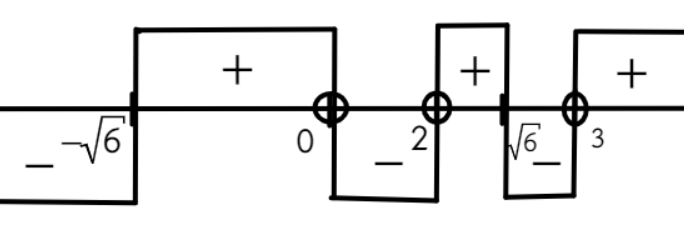
\includegraphics[scale=0.35]{int42.png}}
\end{figure}
$x\in[-\sqrt{6};0)\cup(2;\sqrt{6}]\cup(3;+\infty).$\\
